%================================================================
\section{Project plan}\label{sec:project_plan}
%================================================================
\begin{enumerate}
    \item Decide on theoretical background, such as articles and machine learning methods.
    \item Decide on environment setup and generate synthetic data using \verb|RatInABox| \cite{george:2022:ratinabox}
    \item Set up vanilla RNN using \verb|PyTorch| \cite{2017:pytorch}, and experiment with parameters.
    \item Expand experiment to include more complex environments, and/or objects in the environment, and train the model. Test the model on both seen and unseen environments, and compare performance.
\end{enumerate}


%================================================================
\section{Progress report}\label{sec:progress_report}
%================================================================
I researched the use of neural networks, specifically recurrent neural networks (RNN), and decided to look more into path integration. As a main article I will focus on the work of Banino et al. in \cite{banino:2018:vector_based}.

To generate synthetic trajectories of an agent moving in an environment, similar to a rodent exploring a new environment, I used a package called \verb|RatInABox|. I started with a default square environment of $1 \times 1$ meter, and an agent with no bias toward walls. With this setup I generated a dataset containing velocity and position.

Next, I started building the RNN model. I did some test runs using a basic RNN from PyTorch, however, it was not able to learn the correct path. I continued building a vanilla RNN using the module class provided by PyTorch, and set up a model which was able to predict similar trajectories as the labeled trajectories. 

So far I have tested the model using a hidden layer with 7 and 10 neurons, increasing the number of neurons also increase the accuracy. I have also tested with different number of epochs, batch sizes and learning rates during implementation. Figure \ref{fig:test_model} shows the current model predictions.
\begin{figure}[H]
    \centering
    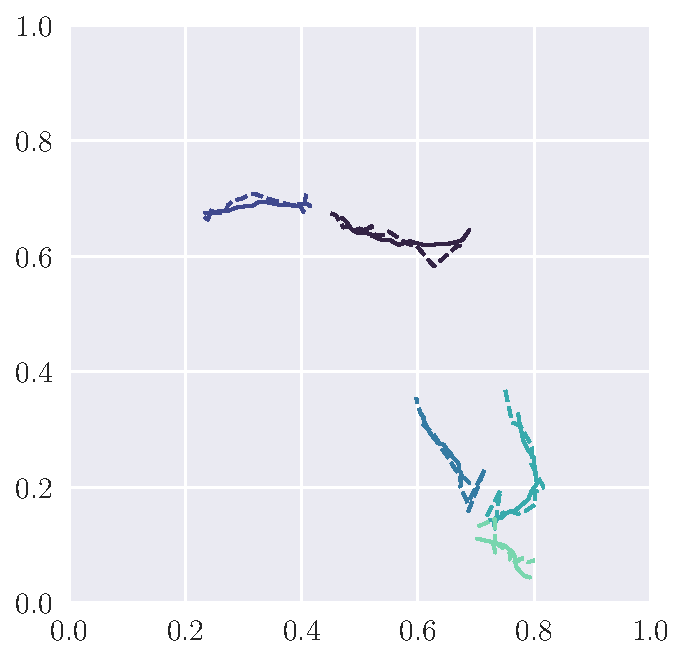
\includegraphics[width=\linewidth]{project/latex/figures/test_model.pdf}
    \caption{The model have been trained on 5 different sequences, each with 19 time steps. The original trajectories, are plotted in solid lines, and the predicted trajectories in dashed lines. }
    \label{fig:test_model}
\end{figure}


%================================================================
\section{Future work}\label{sec:future_work}
%================================================================
The next step is to tune the model, and investigate different parameters such as learning rate and optimizers. Continuing, I will experiment with different environments, and agent biases. And if time allows, I will test the model on unseen environments. In addition, I plan on training a model on synthetic and test it on experimental data. 